% !TEX root = ../Lazcorreta.Tesis.tex
\ABIERTO

%Los trabajos expuestos en los capítulos anteriores muestran una dificultad presente en muchas investigaciones en el ámbito de la informática, la imposibilidad de comprobar si los resultados obtenidos son correctos y aplicables con la tecnología actual. Todas las Ciencias recogen una Teoría que la sustenta, la Informática también, pero las demostraciones teóricas basadas en otras Ciencias no siempre son válidas para la Informática. Hay muchos artículos teóricos sobre Minería de Datos, pero algunos de ellos no evolucionan en un artículo posterior que muestre cómo se ha realizado el experimento con la tecnología actual usando datos reales.
%
%Es fácil calcular teóricamente el número de reglas de asociación presente en una colección concreta de datos, pero si el algoritmo propuesto no es capaz de almacenar en RAM todas las reglas de asociación del problema no servirá de nada ese algoritmo en esa situación. \texttt{mushroom} fue el primer caso que encontré curioso en el ambicioso campo de la Minería de Datos, una colección de tan solo 5\,644 registros de 23 valores que sólo contenía 100 valores diferentes no podía ser analizada a fondo por el mejor algoritmo de ARM que conozco, Apriori, cuando el número de transacciones distintas que se puede obtener bajo estas circunstancias es X\,XXX\,XXX y con ellas tenemos un máximo de X\,XXX\,XXX\,XXX\,XXX reglas de asociación. La tecnología actual de un equipo de escritorio no puede gestionar en RAM tanta información, pero me negaba a creer que no se pudiera extraer \emph{toda la información} que contuviera un problema tan pequeño. Al profundizar en \texttt{mushroom} y los artículos que lo mencionaban y otras colecciones de datos que encontré publicadas en los mismos portales encontré un modo de indicar al algoritmo de ARM que estoy tratando con un tipo de colecciones de datos especial. No es simplemente una colección de transacciones como las analizadas en~\ref{sec:arm:conceptos-basicos} si no que éstas tienen unas restricciones muy fuertes en su definición.
%
%Este informe refleja el trabajo que he realizado para descubrir lo suficiente como para ser merecedor del título de doctor en Informática. Los anteriores capítulos reflejan una gran labor de documentación y exposición científica de los resultados que podía obtener con colecciones de datos fijas, no disponía de un servidor capaz de poner a prueba nuestras aportaciones y realizar sugerencias en tiempo real a un gran número de usuarios. Podía comprobar que mis cálculos se podían realizar con la tecnología actual y las colecciones de datos que yo manejaba pero no sabía qué ocurriría si aumentaran mis colecciones de datos o si pudiera realizar sugerencias en tiempo real. Es un buen trabajo teórico apoyado en algunas realizaciones prácticas pero del que no puedo extraer aún la conclusión que es un buen trabajo de investigación en Informática.

Uno de los problemas de la búsqueda de \ars mediante equipos informáticos es su necesidad de memoria RAM para guardar todos los \itemsets frecuentes (\aprioriL) en un lugar de rápido acceso para ser más eficientes en la búsqueda de \ars. El \dilemaIR puede aparecer en cualquier momento, dependiendo de los datos que contenga el almacén \D que estemos analizando, y se siguen proponiendo ideas para aliviarlo como el uso de umbrales automáticos para el \soporte propuesto por~\citet{SadhasivamAngamuthu-MiningRareItemsetWithAutomatedSupportThresholds-2011}. Sería interesante poder averiguar, en base a información básica del fichero \D, qué requisitos de memoria RAM necesitamos, de cuáles disponemos y, con ello, deducir hasta qué \soporte mínimo podemos trabajar con esa colección específica de datos en este equipo en particular. Hay estudios sobre ello [cita sobre \mushroom de gAcademy]. Aunque este proceso puede llevar algo de tiempo (y restar eficiencia global al algoritmo de \FIM) permite ahorrar el tiempo perdido cuando el programa deja de funcionar por falta de RAM y no es capaz de ofrecernos ningún resultado.

%TODO: Reorganizar, algo de esto se menta en el primer párrafo
%TODO: Ojo, el enlace queda en un salto de página y afecta a la cabecera de la siguiente página. COMPROBARLO EN LA VERSIÓN FINAL
Esta reflexión nos llamó la atención en ficheros tan "`pequeños"' como \mushroom o \texttt{chess.dat}. \mushroom es una colección de datos ampliamente utilizada debido a su publicación en \urlConNotaAlPie{https://archive.ics.uci.edu/ml/datasets/Mushroom}{UCI - Machine Learning Repository}, donde podemos encontrar una completa descripción de los datos en sí y de su aparición en el mundo de la investigación. Encontramos información sobre el uso de este almacén \D en artículos de \clasificacion.

%TODO: Revisar esta información
La Minería de Reglas de \Clasificacion (CRM) toma pronto las bondades de la Minería de Reglas de Asociación (ARM) derivando en una nueva línea de investigación en auge denominada Minería de Reglas de Clasificación Asociativa (CARM) ~\citep{LiuHsuMa-IntegratingClassificationAndARM-1998, Bayardo-EfficientlyMiningLongPatternsFromDB-1998, WangXinCoenen-MiningEfficientlySignificantCAR-2008} donde se aprovecha el potencial que tienen las \ars para descubrir clasificadores precisos.\borrar{Añadir más citas}

%TODO: Añadir ZakiPetersAssentSeidl_Clicks_06 y Ziani:Ouinten:MiningMaximalFIJavaImplOfFPMAXalgorithm:09 (dea.bib) 
Estos ficheros han sido analizados en muchos artículos desde el punto de vista de la \arm clásica~\citep{Suzuki-DiscoveringInterestingExceptionRulesWithRulePair-2004, Borgelt-EfficientImplementationsOfAprioriAndEclat-2004, ThabtahCowlingHammoud-ImprovingRuleSorting-2006, WangXinCoenen-MiningEfficientlySignificantCAR-2008, LiZhang-MiningMaximalFIOnGraphicsProcessors-2010, MalikRaheja-ImprovingPerformanceOfFrequentItemsetAlgorithm-2013, RituArora-IntensificationOfExecutionOfFrequentItemSetAlgorithms-2014, SahooKumarGoswami-AnAlgorithmForMiningHighUtilityClosedItemsetsAndGenerators-2014}. Se proponen nuevas medidas, como la \emph{utilidad} de los \itemsets~\citep{WuShie-MiningTopKHighUtilityItemsets-2012} para aliviar el \dilemaIR. En todos los casos se ha de recurrir al \soporte mínimo para poder llevar a cabo el análisis en un tiempo prudencial (algo más de 2 segundos en el caso de~\citeauthor{RituArora-IntensificationOfExecutionOfFrequentItemSetAlgorithms-2014}, un estudio muy reciente cuyos gráficos coinciden con los de~\citeauthor{MalikRaheja-ImprovingPerformanceOfFrequentItemsetAlgorithm-2013}). Intentamos aplicar técnicas de \dm a colecciones relativamente pequeñas (\mushroom sólo contiene $8\,124 \times 23$ datos) y no podemos profundizar o trabajar en tiempo real si no aplicamos recortes drásticos de información. Hoy en día, almacenes \D de este tamaño deberían poder analizarse en tiempos razonables sin prescindir de ninguno de sus datos.

La Minería de Reglas de Clasificación Asociativa (CARM) transforma los datasets que han de ser analizados desde la perspectiva de CRM para que puedan ser vistos como conjuntos de transacciones y hacer un análisis basado en ARM. Para ello convierten los valores utilizados en CRM, formado por pares atributo=valor, en atributos binarios que tendrán el significado ``Si aparece el atributo binario X entonces el registro toma el valor Y en el atributo original $\A_i$''. Ha habido grandes avances en \Clasificacion gracias a esta pequeña transformación, sin embargo también se ha perdido información muy importante sobre el dataset en estudio, que no será aprovechada si no la incorporamos a la colección de transacciones que queremos analizar con ARM.\borrar{Mejorar}

Antes de obtener información sobre \mushroom comenzamos a analizar los resultados obtenidos en nuestros propios experimentos sobre este almacén \D. Al observarlos encontramos una estructura concreta: todas las filas ("`\transacciones"') tienen el mismo número de datos y en la primera columna sólo aparece un 1 o un 2, en la segunda sólo un 3, 4 o 5\ldots Se trata de una estructura muy rígida y con exceso de información. Al descubrir que el 1 aparecía en X\,XXX \transacciones dedujimos que el 2 aparecería en las restantes 8\,124 - X\,XXX. En el proceso de \fim estábamos desperdiciando esta información y nos entreteníamos en contar el número de veces que aparecía el ítem 2. También descubrimos que el ítem 3 aparecía en un total de Y\,YYY \transacciones, en Z\,ZZZ ocasiones junto al ítem 1, luego en las restantes Y\,YYY - Z\,ZZZ veces que aparece ha de estar junto al ítem 2. No necesitamos averiguar nada sobre el ítem 2, lo que averigüemos sobre el ítem 1 nos dará toda la información que tiene \D sobre el ítem 2. No necesitamos utilizar memoria RAM para guardar información sobre el ítem 2, tendremos memoria RAM libre para analizar los \irs más frecuentes de \D.

Tras llevar a cabo la investigación que se expone en este capítulo podemos afirmar que, aunque todas las citas usadas en los párrafos anteriores han experimentado con \mushroom para aliviar su \dilemaIR, \mushroom y muchas colecciones de datos de similares características realmente no contienen \IRs.


\cite{Lichman-UCI-2013} ponen a disposición de investigadores una buena colección de datos. Con ellos podemos probar nuestras propuestas y, lo que es más importante, hacer comparaciones con otros trabajos ya publicados, en situaciones similares y con los mismos datos. Aunque esto no siempre es así, muchos de los experimentos relatados en la amplia bibliografía de esta tesis han usado aparentemente los mismos datos pero al profundizar en ellos observamos pequeñas diferencias que pueden alterar los resultados de las comparaciones llevadas a cabo. En la sección~\ref{sec:clasificacion:datos-missing} mostraremos un caso en el que los autores modifican los datos originales, lo que nos llevó a experimentar con dos datasets distintos diseñados para el mismo problema de \clasificacion y nos permitió llegar a conclusiones interesantes que de otro modo quizá no habríamos descubierto.


 % \citet{Freitas:UnderstandingDiffBetweenClassifAndDiscoveryOfAR:00} muestran las diferencias existentes entre \ac{ARM} y la tarea de \clasificacion. El debate se debe a que muchas de las investigaciones sobre \ac{ARM} presentan sus resultados como si se tratara de tareas de \clasificacion cuando en realidad no son tales. Estas diferencias nos permiten ver analogías existentes entre ambas tareas que permiten una adaptación de la información extraída de los algoritmos de búsqueda de reglas de asociación para la tarea de \clasificacion, como muestran \citet{Liu:Hsu:Ma:IntegratingClassAndARM:98} en su artículo. La primera diferencia que destacan es a nivel sintáctico: las reglas de asociación muestran en su \consecuente un conjunto de ítems mientras que la tarea de \clasificacion sólo debe mostrar como \consecuente la clase a la que pertenece el individuo (transacción) en estudio. Otra diferencia es la simetría respecto a los elementos incluidos en \antecedente y \consecuente, las reglas de asociación son simétricas si sólo nos fijamos en que tanto \antecedente como \consecuente están formados por ítems (atributos), mientras que en \clasificacion el \antecedente lo forman ítems y el \consecuente es siempre una clase de pertenencia. En consecuencia, las reglas de asociación deben ser del tipo $X\rightarrow y$, donde $X$ es un conjunto de ítems (atributos y no clases) e $y$ es la clase a la que pertenece la transacción que contiene $X$, para poder ser utilizadas en tareas de \clasificacion. Esto no parece suficiente para los autores debido al modo de operar de los algoritmos de \clasificacion: en una primera fase de entrenamiento se encuentran las reglas de \clasificacion entre individuos previamente clasificados, lo que constituye información del ``pasado'' de la población en estudio, mientras que la segunda fase se utiliza para clasificar los individuos del ``presente'' o ``futuro'' según las reglas encontradas en la primera fase. En \ac{ARM} no existe \clasificacion previa ni entrenamiento, y todos los individuos en estudio pertenecen a una misma cohorte, el ``presente'', que en muchas situaciones pretende ser utilizado para inferir las reglas que se cumplirán en el ``futuro''. Esto nos lleva a pensar que el uso de reglas de asociación en tareas de \clasificacion puede realizarse si existe una transformación adecuada de la información obtenida en el proceso de \ac{ARM} -- relaciones existentes entre los ítems de un conjunto de transacciones -- en la información necesaria para clasificar los individuos en estudio -- clases de pertenencia y reglas de \clasificacion.




\section{Conceptos básicos}
\label{sec:clasificacion:conceptos-basicos}
% !TEX root = ../../Lazcorreta.Tesis.tex
%TODO: Incluir \CAR en el índice como Regla de Clasificación Asociativa o Regla de Asociación de Clases (estudiarlo mejor en la literatura, esta última sólo me suena del proyecto de tesis de H.León).
El problema de \Clasificacion tiene ya su propia notación, igual que el de \arm (definida en el capítulo~\ref{chap:arm}), en esta sección intentaremos unificarla y discutiremos algunos aspectos de ambas disciplinas que no han sido considerados en la bibliografía usada para este trabajo, lo que nos llevará también a definir nuevos conceptos e intentar caracterizarlos.


\begin{Definition}[Individuo]
   Sean $A_i, i = 1 \ldots n$ un conjunto de atributos, siendo $n_i$ el número de valores distintos que puede tomar el atributo $A_i$. Definimos un \emph{individuo} como una $n$-túpla, un conjunto de $n$ valores obtenidos ordenadamente de los atributos $A_i$.
   $$individuo = \left(a_1, a_2\ldots a_n\right), a_i \in A_i$$
\label{def:individuo}
\end{Definition}






\subsection{Tal}
\label{sec:clasificacion:conceptos-basicos:tal}
%\input{contenido/clasificacion/conceptos-basicos/tal}

\begin{Definition}[Individuo]
   Sean $A_i, i = 1 \ldots n$ un conjunto de atributos, siendo $n_i$ el número de valores distintos que puede tomar el atributo $A_i$. Definimos un \emph{individuo} como una $n$-túpla, un conjunto de $n$ valores obtenidos ordenadamente de los atributos $A_i$.
   $$individuo = \left(a_1, a_2\ldots a_n\right), a_i \in A_i$$
\label{def:individuo}
\end{Definition}


\begin{Definition}[Registro]
   Sean $A_i, i = 1 \ldots n$ un conjunto de atributos, siendo $n_i$ el número de valores distintos que puede tomar el atributo $A_i$. Definimos un registro como una $n$-túpla, un conjunto de $n$ valores obtenidos ordenadamente de los atributos $A_i$.
   $$registro = \left(item_1, item_2\ldots item_n\right), item_i \in A_i$$
\label{def:registro}
\end{Definition}

\begin{Definition}[\Catalogo] Un \catalogo es un conjunto de $N$ registros diferentes.
   $$\catalogo = \left\{registro_i, i = 1\ldots N\ | \ registro_i \neq registro_j \forall i \neq j\right\}$$
\label{def:catalogo}
\end{Definition}







\section{\Catalogo}
\label{sec:clasificacion:catalogo}
% !TEX root = ../../Lazcorreta.Tesis.tex
\ABIERTO

\begin{wrapfigure}{o}{0.24\textwidth}
  \centering
  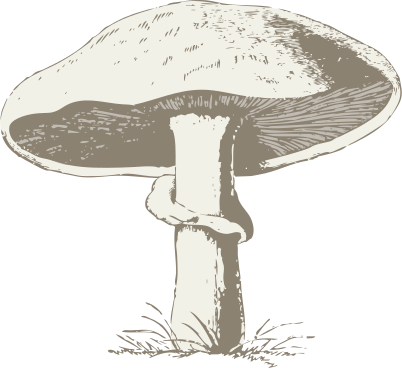
\includegraphics[width=.24\textwidth]{johnny_automatic_mushroom.pdf}
	\caption{Seta (\mushroom)}
	\label{fig:Seta}
\end{wrapfigure}
Al revisar la documentación sobre \mushroom\footnote{Ilustración obtenida en \url{https://openclipart.org/detail/900/two-mushrooms-by-johnny_automatic}} pudimos plantear mejor el problema que queríamos resolver, encontrar todas las \ARs presentes en un fichero "`pequeño"' que presenta estas características. En \href{https://archive.ics.uci.edu/ml/datasets/Mushroom}{UCI - Machine Learning Repository}\footnote{\url{https://archive.ics.uci.edu/ml/datasets/Mushroom}} describen su origen como



\selectlanguage{english}
\begin{quote}
   Mushroom records drawn from The Audubon Society Field Guide to North American Mushrooms (1981). G. H. Lincoff (Pres.), New York: Alfred A. Knopf 
\end{quote}
\selectlanguage{spanish}
\noindent Describen brevemente el contenido del fichero, indicando que se trata de setas clasificadas como comestibles o venenosas (primer valor de cada fila).
\selectlanguage{english}
\begin{quote}
\label{cita:incertidumbre-suprimida-en-mushroom}
   This data set includes descriptions of hypothetical samples corresponding to 23 species of gilled mushrooms in the Agaricus and Lepiota Family (pp. 500-525). Each species is identified as definitely edible, definitely poisonous, or of unknown edibility and not recommended. This latter class was combined with the poisonous one. The Guide clearly states that there is no simple rule for determining the edibility of a mushroom; no rule like ``leaflets three, let it be'' for Poisonous Oak and Ivy.
\end{quote}
\selectlanguage{spanish}
\noindent Y explican los valores que puede tomar cada uno de los atributos.
\selectlanguage{english}
\begin{quote}
   \footnotesize
   1. cap-shape: bell=b, conical=c, convex=x, flat=f, knobbed=k, sunken=s
   
   2. cap-surface: fibrous=f, grooves=g, scaly=y, smooth=s

   3. cap-color: brown=n, buff=b, cinnamon=c, gray=g, green=r, pink=p, purple=u, red=e, white=w, yellow=y

   4. bruises?: bruises=t, no=f

   5. odor: almond=a, anise=l, creosote=c, fishy=y, foul=f, musty=m, none=n, pungent=p, spicy=s

   6. gill-attachment: attached=a, descending=d, free=f, notched=n

   7. gill-spacing: close=c, crowded=w, distant=d

   8. gill-size: broad=b, narrow=n

   9. gill-color: black=k, brown=n, buff=b, chocolate=h, gray=g, green=r, orange=o, pink=p, purple=u, red=e, white=w, yellow=y

   10. stalk-shape: enlarging=e, tapering=t

   11. stalk-root: bulbous=b, club=c, cup=u, equal=e, rhizomorphs=z, rooted=r, missing=?

   12. stalk-surface-above-ring: fibrous=f, scaly=y, silky=k, smooth=s

   13. stalk-surface-below-ring: fibrous=f, scaly=y, silky=k, smooth=s

   14. stalk-color-above-ring: brown=n, buff=b, cinnamon=c, gray=g, orange=o, pink=p, red=e, white=w, yellow=y

   15. stalk-color-below-ring: brown=n, buff=b, cinnamon=c, gray=g, orange=o, pink=p, red=e, white=w, yellow=y

   16. veil-type: partial=p, universal=u

   17. veil-color: brown=n, orange=o, white=w, yellow=y

   18. ring-number: none=n, one=o, two=t

   19. ring-type: cobwebby=c, evanescent=e, flaring=f, large=l, none=n, pendant=p, sheathing=s, zone=z

   20. spore-print-color: black=k, brown=n, buff=b, chocolate=h, green=r, orange=o, purple=u, white=w, yellow=y

   21. population: abundant=a, clustered=c, numerous=n, scattered=s, several=v, solitary=y

   22. habitat: grasses=g, leaves=l, meadows=m, paths=p, urban=u, waste=w, woods=d
\end{quote}
\selectlanguage{spanish}

\noindent El fichero \mushroom\footnote{\url{https://archive.ics.uci.edu/ml/machine-learning-databases/mushroom/agaricus-lepiota.data}} es un fichero de texto con 8\,124 líneas, de las que muestro aquí las tres primeras:
\begin{quote}
   \footnotesize
   p,x,s,n,t,p,f,c,n,k,e,e,s,s,w,w,p,w,o,p,k,s,u
   
   e,x,s,y,t,a,f,c,b,k,e,c,s,s,w,w,p,w,o,p,n,n,g
   
   e,b,s,w,t,l,f,c,b,n,e,c,s,s,w,w,p,w,o,p,n,n,m
\end{quote}

\noindent El fichero \mushroom con el que llevo años trabajando está codificado de otro modo, conteniendo la misma información
\begin{quote}
   \footnotesize
   1 3 9 13 23 25 34 36 38 40 52 54 59 63 67 76 85 86 90 93 98 107 113
   
   2 3 9 14 23 26 34 36 39 40 52 55 59 63 67 76 85 86 90 93 99 108 114
   
   2 4 9 15 23 27 34 36 39 41 52 55 59 63 67 76 85 86 90 93 99 108 115
\end{quote}

Este modo de registrar información sobre los individuos de una población es muy habitual en todas las ciencias. Se determina qué \atributos se pueden medir, codificándolos mediante un número reducido de valores distintos, se observa a un \emph{individuo} y se mide el valor que toma en cada uno de los atributos seleccionados, obteniendo un vector de códigos.

\begin{Definition}[Individuo]
   Sean $A_i, i = 1 \ldots n$ un conjunto de atributos, siendo $n_i$ el número de valores distintos que puede tomar el atributo $A_i$. Definimos un \emph{individuo} como una $n$-túpla, un conjunto de $n$ valores obtenidos ordenadamente de los atributos $A_i$.
   $$individuo = \left(a_1, a_2\ldots a_n\right), a_i \in A_i$$
\label{def:individuo}
\end{Definition}

El propósito de recoger esta información suele ser el de \clasificacion, clasificar al \emph{individuo} en función de los valores observados en los atributos en estudio. Esta asignación se hace en función de la información que tenemos sobre esta población, generalmente un almacén \D como \mushroom, que contiene datos sobre muchos individuos de esta población correctamente clasificados.

Aunque es un problema de \Clasificacion se trata usando \arm por la forma en que se han codificado los valores expuestos para crear el fichero \mushroom. Se han utilizado números enteros consecutivos, los dos primeros para determinar la \clase (1 = \emph{venenosa}, 2 = \emph{comestible}), los siguientes para anotar el valor del atributo \texttt{cap-shape} (3 = \emph{convex}, 4 = \emph{bell}, 5 = \emph{sunken}, 6 = \emph{flat}, 7 = \emph{knobbed}, 8 = \emph{conical}), a continuación los valores del atributo \texttt{cap-surface} (9 = \emph{smooth}, 10, 11 y 12)\ldots Si encontramos \ARs fuertes entre los atributos y la \clase podemos intentar clasificar mejor a cualquier individuo de la población.







Esta estructura permite reducir notablemente la información a procesar para extraer reglas de asociación de estos ficheros, lo que convierte su estudio en una mera ejecución con \soporte mínimo nulo (si fueran más grandes podríamos averiguar antes si no están afectados por el \dilemaIR como se ha mencionado antes). Analicemos primero la estructura y veremos después una serie de características. Para entenderlo mejor analizaremos \mushroom, que es quien nos puso sobre la pista de que algo se hacía mal con este tipo de almacenes \D.

\begin{enumerate}
	\item Tiene 8\,124 filas (a las que hemos llamado \transacciones pero llamaremos \emph{registro} a partir de ahora).
	\item Cada registro tiene 23 elementos.
   \item El primer valor de cada registro es un 1 o un 2.
         
         El segundo valor es un 3, 4, 5, 6, 7 u 8.
         
         \ldots
         
         Esto nos hace pensar que cada posición del registro representa a una variable categórica. Y descubrir que los valores utilizados para representar a una variable no coinciden con los utilizados por el resto de variables, y que estos valores son consecutivos, 1\ldots119.
   % \item Si en una fila está el 1, entonces no está el 2. Esto mismo ocurre con los grupos \{3,4,5\}, \{6,7\},\ldots \{118,119\}. Esto nos hace pensar que son los valores de diferentes \atributos o \clases. Cada fila representa el valor que un individuo toma en un determinado atributo o \clase.
\end{enumerate}

%TODO: Esto va más adelante, fuera de la INTRO
En la primera lectura de \D, la que utilizamos para crear \aprioriC[1], podemos anotar la longitud de todas las \transacciones. De este modo será muy fácil comprobar si estamos trabajando con un \catalogo.

Esto sólo lo detectamos porque se han codificado los valores de cada variable categórica de modo que no haya dos iguales y sean todos consecutivos. Basta con aplicar el algoritmo mostrado en el listado~\ref{listado:comprobarCatalogo} para averiguar si \D contiene un \catalogo, una vez leído y obtenido \aprioriC[1] y $M$, el número de valores observado en todas las \transacciones.

\lstinputlisting[label=listado:comprobarCatalogo,
                 caption={Comprobación sobre \catalogos},
                 float=htb,
                 basicstyle=\footnotesize]
                 {./contenido/clasificacion/codigo/algComprobarCatalogo}


   % \item No hay dos registros iguales. Esto nos hace pensar que se trata de un \textbf{\catalogo}, no de una \textbf{muestra}. Aunque en ambos casos la reducción de información a procesar que podemos es la misma (en la muestra\ldots) la información que obtendremos no es la misma, lo que se explica en la sección~\ref{sec:3-3-CatalogoVsMuestra}.

Un \catalogo tiene una estructura muy rígida. Si hay valores missing se puede añadir un valor al atributo en cuestión indicando esa circunstancia, o no utilizar la información del atributo en cuestión o incluso hacer una estimación del valor si se puede justificar.

En un \catalogo todos los registros contienen $n$ datos, y si forma parte de una tarea de \clasificacion uno o varios de esos datos representan una \clase, generalmente el "`\atributo"' cuyo valor queremos determinar a partir de la observación de los valores del resto de \atributos.

\begin{Definition}[Registro]
   Sean $A_i, i = 1 \ldots n$ un conjunto de atributos, siendo $n_i$ el número de valores distintos que puede tomar el atributo $A_i$. Definimos un registro como una $n$-túpla, un conjunto de $n$ valores obtenidos ordenadamente de los atributos $A_i$.
   $$registro = \left(item_1, item_2\ldots item_n\right), item_i \in A_i$$
\label{def:registro}
\end{Definition}

\begin{Definition}[\Catalogo] Un \catalogo es un conjunto de $N$ registros diferentes.
   $$\catalogo = \left\{registro_i, i = 1\ldots N\ | \ registro_i \neq registro_j \forall i \neq j\right\}$$
\label{def:catalogo}
\end{Definition}
% \borrar{Buscar una definición mejor, en \clasificacion}


El número de combinaciones entre todos los valores de los atributos en estudio es muy grande, sin embargo cuando se está haciendo un estudio real no se obtendrán todas las combinaciones posibles. En un \catalogo sólo están las combinaciones que interesa estudiar, básicamente aquellas que sí se dan en la población en estudio. Es una selección de los registros que se podrían formar con todas las combinaciones de valores proporcionada por los atributos en estudio.

La esencia de un \catalogo es que no tiene registros repetidos. Si tomamos una muestra de una población midiendo en cada individuo todos los valores de los atributos del estudio es muy probable que en la muestra existan registros repetidos. Las muestras de este tipo se verán a fondo en la sección~\ref{sec:clasificacion:catalogo:muestras}, es importante estudiar sus diferencias con los \catalogos pues contienen información sensiblemente diferente.

Un \catalogo puede cambiarse fácilmente, basta con cambiar el número de valores que puede tomar una de las variables en estudio para que cambie por completo el \catalogo. Una muestra no puede cambiarse, se obtiene de la realidad, se diseña previamente y si se quiere añadir a otra muestra en que se han utilizado otros valores debería rehacerse\ldots


Si aprovechamos esta información podemos reducir notablemente los ítems a procesar sin perder la información que contiene el \catalogo (o muestra) completo\ldots

% \borrar{Aquí viene el ejemplo de Interacción'12, he de buscar cómo escribir código.}







%\subsection{\Catalogo comprimido}
%\label{sec:3-1-1-CatalogoComprimido}
%\input{./3-ARMCatalogos/3_1_Catalogos/3_1_1_CatalogoComprimido}
%
%
%
%
%
%
%
%\subsection{Lectura de \catalogo comprimido}
%\label{sec:3-1-2-LecturaDeCatalogoComprimido}
%\input{./3-ARMCatalogos/3_1_Catalogos/3_1_2_LecturaDeCatalogoComprimido}
%
%
%










Los catálogos son colecciones de registros preparadas para resolver informáticamente un problema de clasificación. Y muchos investigadores de esta especialidad publican sus datos para que otros investigadores puedan hacer pruebas con las mismas condiciones de partida: una colección de datos con ciertas características. En UCI, KEEL, LUCS\ldots encontraremos muchos catálogos entre los datasets que publican para resolver problemas de clasificación.\marginpar{\footnotesize Acabo de descubrir LUCS, que discretiza las colecciones de UCI y me ofrece 97 valores distintos en adult, frente a los 27\,245 que tiene el de UCI, he de analizarlo con mi código y EXPLICAR MEJOR LAS CONSECUENCIAS DE APLICAR ANTES O DESPUÉS MI MÉTODO O LA AGRUPACIÓN DE VALORES EN ATRIBUTOS NUMÉRICOS ya que se obtendrán reglas y catálogos completos bastante diferentes, esto da para otro artículo y más si tengo en cuenta que tiene datos missing por lo que puedo obtener catálogos completos usando menos atributos con más registros o catálogos completos usando sólo los atributos registrados en cada registro (a no ser que el análisis nos diga que cierto atributo no aporta información\ldots.}

Cuando no sabíamos que esos ficheros contenían catálogos intentábamos aplicar bien conocidos algoritmos de ARM pero no podíamos extraer información que contienen los datos porque se desbordaba la RAM del equipo en que se está aplicando el algoritmo y se abortaba el proceso tras horas de cálculos que finalmente no obteníamos. Esto nos sorprendía porque el primer catálogo que intentamos analizar con Apriori sólo tiene 5\,644 registros de 23 datos, no son números excesivos para un problema de Minería de Datos analizado con un ordenador de escritorio con cierta potencia y capacidad de RAM. Eso nos llevó a descubrir cómo se creó el catálogo a través de \url{UCI/mushroom}\ldots

Los catálogos caracterizan un problema de clasificación concreto. Si queremos plantear otro problema de clasificación, bien etiquetando a los mismos individuos en otras \clases o bien utilizando atributos diferentes no podemos utilizar directamente cualquier catálogo que tengamos sobre la misma población. Si los dos problemas usaran los mismos atributos pero diferentes \clases y las \clases en estudio son independientes no servirá de nada la información que tengamos sobre los catálogos completos del primer problema de clasificación si no sabemos analizar qué información puede ser relevante y cuál no, de hecho la información menos relevante en esta situación es la distribución de las \clases en cada uno de los problemas de clasificación por lo que debemos huir de interpretaciones erróneas utilizando estos datos para estimar soportes o confianzas poblacionales.

De un catálogo se puede extraer información válida para otro problema de clasificación que utilice los mismos atributos ya que si en la muestra en que se basa el catálogo no presenta cierta relación entre los valores de los atributos YA SABEMOS QUE NO APARECERÁ ESA RELACIÓN AUNQUE CAMBIEMOS DE CLASES (siempre que el catálogo sea válido, aún tengo que hacer muchas definiciones sobre muestra, población, distribución de \clases, problema de \clasificacion, \atributos, \clases, \catalogos, catálogos completos, validez de un catálogo\ldots).

Aunque la \ARM busca cualquier relación entre cualquier par (o $k$-itemset) de valores de \D, el objetivo del problema de \clasificacion es siempre el mismo, etiquetar cada \registro con una \clase basándose en la información disponible sobre otros \registros con valores idénticos en sus \atributos.





\subsection{Muestras}
\label{sec:clasificacion:catalogo:muestras}
La importancia que se da en todos los estudios de \ARM al \soporte de una \ar se justifica cuando se trabaja con muestras, que no contienen la misma información que un \catalogo. Para obtener una muestra en un problema de \clasificacion se han de seleccionar individuos de una población, medir en cada uno de ellos el valor que toma cada uno de los \atributos en estudio y averiguar la \clase a la que pertenece. Al guardar todos los \registros obtenidos de este modo es posible que existan \registros repetidos, lo que aporta información sobre la distribución de la población en estudio con un elevado coste sobre los \catalogos ya que en estos no deberíamos repetir el registro si no añadir un número entero indicando el número de veces que aparece el \registro en la muestra.











\section{\Catalogo Comprimido}
\label{sec:catalogos:catalogo-comprimido}
% !TEX root = ../../Lazcorreta.Tesis.tex
\ABIERTO
% !TEX root = ../../../Lazcorreta.Tesis.tex
\ABIERTO

Un \catalogo comprimido contiene en muy poco espacio la misma información que un \catalogo.
\begin{itemize}
   \item $N$, el número de registros del \catalogo.
   \item Los valores correspondientes a cada atributo junto a su frecuencia en el \catalogo (\aprioriC[1] ampliado con información de $A_i$).
   \item Los valores menos frecuentes de cada atributo.
\end{itemize}

Con esta información es inmediato reconstruir el \catalogo original, pero no necesitaremos hacerlo ya que vamos a trabajar con el \catalogo comprimido y la información extra disponible. De hecho esta información nos permitirá crear el árbol \aprioriL completo antes de comenzar a hacer la segunda lectura de \D, esta vez a través del \catalogo comprimido.

En primer lugar no estamos interesados en crear un árbol \aprioriL completo, este era uno de los problemas que provocó la búsqueda de algoritmos eficientes para \ARM. Sólo necesitamos expandir las primeras ramas del árbol, las correspondientes a los valores de la clase. Si necesitáramos cualquier otro valor del árbol completo podríamos reproducirlo con unos pocos cálculos aplicados sobre los datos que contiene nuestro \aprioriL reducido.

Es de destacar que al codificar los datos originales para construir un \catalogo se comenzó con los valores de la clase y a continuación se añadieron los atributos, sin aparente orden. El orden en que estén estos atributos podría ser relevante en un análisis clásico de \arm, podría provocar muchas más búsquedas de las necesarias si la codificación fuera otra. En el caso de los \catalogos comprimidos este hecho no afecta a la eficiencia del algoritmo ni a los recursos empleados. Desde el primer momento se reservará memoria para las primeras ramas del árbol \aprioriL completo y desde entonces no habrá reserva ni destrucción de memoria. El efecto inicial es un alto consumo de memoria que realmente no será utilizada (la que es evitaba reservar a la hora de generar candidatos por la propiedad \apriori). Sin embargo este consumo de memoria será compensado por dos factores: si una hoja de nuestro árbol \aprioriL reducido queda con \soporte nulo hemos descubierto una \emph{Regla de Asociación Negativa}, y ahorramos millones de operaciones de búsqueda a cambio de operaciones de cálculo mucho más adaptadas al trabajo de un procesador.








%TODO: Esto no va aquí, primero hablar de \catalogos -> comprimidos -> apriori_estático -> L
En el listado~\ref{alg:apriori-L-completo} se muestra el árbol \aprioriL completo para cualquier almacén \D basado en la clase \{1,2\} y los atributos \{3,4,5\}, \{6,7\}. Son necesarios 127 nodos para representar todas las posibles combinaciones entre los valores 1 y 7.

\afterpage{\clearpage}
\lstinputlisting[label=alg:apriori-L-completo,
                 caption={\aprioriL completo},
                 float=htb,
                 basicstyle=\scriptsize]
                 {./contenido/clasificacion/codigo/aprioriLcompleto}


Simplemente aplicando la característica\borrar{¿nombre?}\ldots reducimos notablemente el tamaño de \aprioriL, como muestra el listado~\ref{alg:apriori-L-reducido}. Como en un registro no pueden aparecer dos valores de una misma clase o atributo no encontraremos nunca los \itemsets (1,2), (3,4), (3,5), (4,5) y (6,7) por lo que sólo necesitamos 35 nodos para tener la misma información sobre reglas de asociación que contiene la colección de datos que estamos tratando. 

Los

\afterpage{\clearpage}
\lstinputlisting[label=alg:apriori-L-reducido,
                 caption={\aprioriL reducido},
                 float=htb,
                 basicstyle=\scriptsize]
                 {./contenido/clasificacion/codigo/aprioriLreducido}

Por último, si observamos\borrar{¿qué?} \ldots vemos que toda la información que se puede guardar en el árbol \aprioriL reducido mostrado en el listado~\ref{alg:apriori-L-reducido} se puede comprimir de modo que sólo sean necesarios 11 nodos, los mostrados en el listado~\ref{alg:apriori-L-compacto}. El árbol \aprioriL compacto se puede expandir con simples cálculos numéricos hasta obtener el árbol \aprioriL completo si fuera necesario obtener todos sus nodos, lo habitual es que sólo queramos obtener el valor almacenado en un nodo del árbol \aprioriL completo y no sea necesario recrear todo el árbol, aunque tenemos la capacidad de obtener toda la información que contiene. Este formato se ha de tener en cuenta a la hora de leer \D.

Al ser de reducido tamaño es fácil transmitir \catalogos comprimidos entre distintos dispositivos, lo que facilitaría su procesamiento por el dispositivo que ha recibido los datos sin necesidad de mayor interacción. Lo que hay que conseguir son estructuras y métodos adecuados para el procesamiento de estos ficheros usando pocos recursos.

En muchos casos el número de nodos del árbol reducido puede ser mayor que el obtenido con el algoritmo original. Sin embargo sólo estamos guardando el \soporte en cada nodo por lo que no guardamos ni el ítem que tiene ese \soporte (8, 16 o 32 \texttt{bits}) ni el puntero a su hermano menor (32 o 64 \texttt{bits}) por lo que el hecho de contener más nodos no garantiza que se necesite más memoria RAM para guardar su contenido. Sustituir búsquedas por cálculos sobre índices reducirá mucho el tiempo de ejecución del algoritmo.

\afterpage{\clearpage}
\lstinputlisting[label=alg:apriori-L-compacto,
                 caption={\aprioriL compacto},
                 float=htb,
                 basicstyle=\scriptsize]
                 {./contenido/clasificacion/codigo/aprioriLcompacto}











En un fichero con $n$ valores distintos distribuidos en $A$ atributos se parte de un vector inicial de $n - A$ elementos, de los cuales sólo surgirán ramas de los $n_{A_1} - 1$ primeros si estamos ante un problema de \clasificacion.



\subsection{Lectura de catálogos comprimidos}
\label{sec:clasificacion:catalogo-comprimido:lectura}











\section{\CC}
\label{sec:clasificacion:catalogo-completo}
% !TEX root = ../../Lazcorreta.Tesis.tex
\ABIERTO
Al seguir trabajando con \mushroom encontramos otra versión del mismo dataset en KEEL

http://sci2s.ugr.es/keel/dataset.php?cod=178


\borrar{Necesito definir antes conjuntoDeValoresDeAtributos, quizá en otra sección.}
\begin{Definition}[\CC] Un \CC es un \catalogo sin incertidumbre.
   $$\CC = \left\{registro_i, i = 1\ldots N\ | \ registro_i \neq registro_j \forall i \neq j\right\},  conjuntoValoresAtributos son todos diferentes$$
\label{def:catalogo}
\end{Definition}






\subsection{Colecciones de \CCs}
\label{sec:clasificacion:catalogo-comprimido:colecciones}
%\input{contenido/clasificacion/catalogo-comprimido/colecciones}

Todos los \CCs pueden tener un \CC maximal y diversos \CCs de menores dimensiones. Volviendo al origen de esta investigación, disponemos de un dataset\ldots







%TODO: Añadir \missing al índice alfabético
\section{Datos missing}
\label{sec:clasificacion:datos-missing}
% !TEX root = ../../Lazcorreta.Tesis.tex
\ABIERTO
%TODO: Incluir "datos missing" en indice-alfabetico
\mushroom contiene 8\,124 registros en su dataset original de la UCI, sin embargo en el fichero KEEL con el que hemos trabajado desde la sección~\ref{sec:catalogo:catalog} contiene sólo 5\,644 registros porque se han eliminado los \registros con datos missing que contenía el fichero original. Para diferenciar ambos \datasets llamaremos \texttt{mushroom-original} al \dataset de la UCI y \texttt{mushroom-reducido} al que no contiene datos missing.

En un problema de \dm los datos missing no deberían ser considerados. El objetivo de esta disciplina es la obtención de información (previamente desconocida) a partir de los datos. Un dato missing no aporta información como dato, podría ser interpretado en muchos experimentos el hecho de no conocer ese dato pero el dato en sí no lo conocemos y, por lo tanto, no podemos usarlo. Se podrían estimar a partir de los datos que sí conocemos pero si no hay una justificación suficientemente poderosa no deberíamos "`inventar"' ningún valor cuando queremos obtener la información que contienen los datos que realmente conocemos. La \dm se aplica a los datos conocidos o estimados pero en este momento sólo tenemos datos missing sin interpretar por lo que no nos pueden dar ningún tipo de información.

Cualquier \ar que incluya el ítem \texttt{stalk-root=?} en su antecedente debe ser ignorada ya que su interpretación sería "`\emph{Si no sé qué valor tiene stalk-root entonces\ldots}"'.

%TODO: He cambiado la referencia a catalogo-comprimido por catalogo-completo. Comprobar que es correcto.
En un registro, la ausencia de un dato provocará tener un valor menos, lo que traducido a transacciones se convierte en una transacción de distinto tamaño que el resto de registros. Esto sería un problema para tratarlo como se ha propuesto en la sección~\ref{sec:clasificacion:catalogo-completo} ya que el fichero \D no será considerado \catalogo por no tener todos sus registros el mismo tamaño. Una solución consiste en considerar el valor missing de un atributo como un valor distinto al resto de los que realmente contiene, en el caso de \mushroom se denota con \texttt{?}, al convertirlo en fichero \D se codificará ese valor como un valor distinto del atributo al que pertenezca y la única consecuencia es, aparentemente, que tenemos un ítem diferente más.

Los datos missing son difíciles de interpretar correctamente ya que para convertir los ficheros en formato adecuado para ARM se utiliza un código binario para indicar esta situación, i.e., si un registro no contiene información sobre un atributo se crea la categoría ficticia "`dato desconocido"' en dicho atributo y se le asigna esa categoría, así podemos aplicar con cierta normalidad las técnicas de ARM, aunque la interpretación de las reglas que se pueden obtener es confusa:

\begin{quote}
Si no conocemos el valor del atributo $\A_i$ podemos deducir que\ldots
\end{quote}

Eliminar los registros con datos missing parece una estrategia correcta para no tener que gestionar estas \ars. Sin embargo perdemos información sobre 2\,480 registros, sin saber si la información que perdemos es relevante o no lo es.

Si analizamos el fichero \mushroom observaremos que sólo un atributo contiene datos missing, \texttt{stalk-root}, y ya hemos visto en la sección~\ref{sec:clasificacion:catalogo-completo} que este atributo es prescindible, al menos en el dataset reducido de KEEL. Con lo que ahora sabemos sobre \catalogos podemos diseñar otra estrategia, eliminar el atributo \texttt{stalk-root} del dataset original y comprobar si esos 2\,480 registros ignorados por la estrategia utilizada contienen información que habíamos perdido irremediablemente.

En \urlConNotaAlPie{http://sci2s.ugr.es/keel/dataset.php?cod=178}{KEEL - Mushroom} proporcionan dos ficheros \mushroom:
\begin{itemize}
  \item por defecto el que han elaborado con su formato tras eliminar los registros con datos missing, con 5\,644 registros\footnote{\scriptsize\url{http://sci2s.ugr.es/keel/dataset/data/classification/mushroom.zip}},
  \item si lo buscamos nos ofrecen el dataset original en formato KEEL, con 8\,124 registros\footnote{\scriptsize\url{http://sci2s.ugr.es/keel/dataset/data/missing/mushroom.zip}}.
\end{itemize}
Al analizar ambos ficheros se obtienen los siguientes resultados:
\begin{enumerate}
  \item \texttt{mushroom-original} contiene un \sCC de 8\,124 \registros, con un atributo que contiene datos missing, \texttt{stalk-root}, que es prescindible y no aumenta el tamaño del \catalogo.
  \item \texttt{mushroom-reducido} contiene un \sCC de 5\,644 \registros, \texttt{stalk-root} es prescindible y no aumenta el tamaño del \catalogo.
\end{enumerate}
Luego tenemos dos análisis sobre dos \datasets que ofrecen datos similares pero deben contener diferente información. Analizar sus similitudes y diferencias nos dará más información que la que obteníamos con el primer fichero KEEL. Destaquemos que:

\begin{enumerate}
  \item Ambos ficheros son \sCCs. Todos sus \registros son distintos y no contienen incertidumbre.
  \item Si eliminamos en cualquiera de ellos el atributo \texttt{stalk-root} no se reduce el \catalogo ni se pierde información. No sabemos si \texttt{mushroom-reducido} seguirá siendo un \sCC.
\end{enumerate}
Si no sobran los 2\,480 registros de más que tiene el \CC original deberían de aportar algo de información que no está presente en el \catalogo reducido. Esto lo sabremos tras eliminar su atributo \texttt{stalk-root} y comprobar si genera incertidumbre\borrar{Explicarlo con ecuaciones}.
\begin{itemize}
  \item Si no la genera es por\ldots
  \item Si la genera es por\ldots
\end{itemize}



Si eliminamos \texttt{stalk-root} de ambos ficheros obtendremos dos \sCCs distintos, el primero con todos los registros-tipo del segundo y además 2\,480 registros-tipo que no están en el segundo. Es evidente que el primero tiene información más precisa sobre el problema de \clasificacion que estamos analizando. Pero la información extra que contiene no es sobre el atributo \texttt{stalk-root}, ni tan siquiera se utiliza este atributo para obtener esa información, sólo depende de las co-ocurrencias entre valores del resto de atributos. Si eliminamos el atributo \texttt{stalk-root} de ambos ficheros obtendremos dos nuevos \sCCs, esta vez sin datos missing, ambos orientados al mismo problema de \clasificacion y sin ninguna discrepancia entre ellos (de hecho el reducido es una partición del original). Si pudiéramos utilizar cualquiera de ellos en nuestro próximo clasificador está claro que deberíamos usar el \sCC que ese obtiene eliminando el atributo \texttt{stalk-root} al dataset original.

El \sCC mayor contiene al menor pero el menor se ha obtenido a partir de la información proporcionada por otro atributo (que ahora ya no está). Ambos contienen algo de información distinta para el mismo problema de \clasificacion. En el menor hay más $ARN_2$, que desaparecen al añadir nuevos registros-tipo para formar el mayor, es lo que podría ocurrir si seguimos tomando muestras y aparecen nuevos registros-tipo que no presenten incertidumbre, el \sCC va mejorando y nos informa que los datos que conocemos garantizan una buena clasificación (no es necesario medir otro atributo porque no tenemos incertidumbre y cada vez sabemos más sobre los registros-tipo de este problema de clasificación).







No todos los \catalogos con datos missing tendrán las mismas características que \mushroom, pero sí se puede dar en muchos estudios que sigamos añadiendo registros a un dataset pero sin incluir el valor de uno de sus atributos, si el resto de atributos es suficiente para clasificar correctamente al individuo tendremos una situación similar a la analizada en esta sección. Si estamos trabajando con un \sCC completo y válido es muy posible que no necesitemos nunca más medir el valor de ese atributo, pero no deberíamos borrarlo del dataset original porque alguna vez podría aparecer algo de incertidumbre en el \catalogo y sería útil poder añadir toda la información que ya se recogió en su día sobre cualquier otro atributo medible en los individuos en estudio.







\section{Flujos de Datos}
\label{sec:clasificacion:flujos-de-datos}
% !TEX root = ../../Lazcorreta.Tesis.tex
\ABIERTO


%\cite{FMenaHleonHPalancar-ClasificacionBasadaEnCARPAraFlujosDeDatosEstadoDelArte-2013} presentan un estado del arte actualizado sobre el uso de Reglas de Asociación de Clase (CAR) sobre Flujos de Datos, que está estrechamente relacionado con las propuestas hechas en esta sección ya que centran el foco en el \clasificador obtenido tras las primeras lecturas de los datasets disponibles para el estudio de \clasificacion en curso.



%\begin{quote}
%Los \clasificadores para flujos de datos, a diferencia de los \clasificadores para datos estáticos, no disponen de todo el conjunto de transacciones etiquetadas (conjunto de entrenamiento) a priori, sino que estas arriban de forma incremental a lo largo del tiempo. Por otro lado, dado que los flujos de datos son, en teoría, infinitos, resulta imposible cargar todas las transacciones en memoria y se requiere de un algoritmo incremental que actualice el clasificador con la información de las nuevas transacciones, reutilizando la información extraída de las transacciones previas. En general, los clasificadores para flujos de datos [1,8,23] deben garantizar que:
%
%\begin{enumerate}
%  \item Cada \transaccion del flujo de datos sea procesada a lo sumo una vez.
%  \item Los resultados de \clasificacion estén disponibles en todo momento.
%  \item El modelo resultante sea consistente con las nuevas \transacciones que llegan, pues los datos pueden variar a lo largo del tiempo debido a cambios en su distribución de probabilidad.
%\end{enumerate}
%
%La \clasificacion en flujos de datos tiene diversas aplicaciones como: detección de software malicioso [46], \clasificacion de paquetes en el área de las telecomunicaciones [53], monitoreo de procesos industriales [4,37], monitoreo de datos de navegación en vehículos automotrices [38], detección de fraudes en transacciones bancarias [65], entre otros.
%
%Varios han sido los \clasificadores adaptados al entorno de flujos de datos. Entre los más reportados se encuentran los árboles de decisión [19,25,26,34,36,59,61] y los métodos de ensamble de \clasificadores [9,39,47,51,57]. Otros \clasificadores que han recibido menor atención son los basados en el vecino más cercano [5,54], las máquinas de vectores de soporte [43,66] y los basados en reglas. Particularmente, los \clasificadores basados en Reglas de Asociación de Clase (CARs), son preferidos por muchos especialistas debido a su interpretabilidad, aspecto que los hace más expresivos y fáciles de comprender. Su interpretabilidad permite a los especialistas modificar las reglas con base en su experiencia y así mejorar la eficacia del clasificador. Además de los clasificadores basados en CARs, los árboles de decisión también generan reglas comprensibles. Para construir un clasificador utilizando árboles de decisión se sigue una estrategia voraz seleccionando en cada momento la característica que mejor separa las clases. Sin embargo, esta estrategia voraz puede podar reglas interesantes. En [55], los autores probaron que las reglas obtenidas de los árboles de decisión son un subconjunto de las reglas generadas por los clasificadores basados en CARs, asumiendo un umbral relativamente bajo de concurrencia (Soporte) de los elementos que componen la regla.
%\end{quote}

Los \catalogos consiguen reducir el número de objetos a utilizar en memoria RAM, de modo que el \clasificador puede encontrar una \emph{regla determinista basada en los datos conocidos}.\borrar{Añadir \emph{regla determinista basada en los datos conocidos} a definiciones e índice.}








\section{Publicaciones}
\label{sec:clasificacion:publicaciones}
% !TEX root = ../../Lazcorreta.Tesis.tex
En Interacción'12 comenzamos a publicar nuestros resultados sobre las colecciones de \transacciones estructuradas mediante \catalogos. Los mayores avances los hemos obtenido este último año y estamos en un proceso actual de publicación de resultados en diversas revistas y un nuevo congreso internacional.





%\cite{Lazcorreta:Botella:FCaballero:EfficientAnalysisOfTransactionsWebRecommendations:2012}
\subsection*{Efficient analysis of transactions to improve web recommendations, 2012}

\begin{quote}
  Lazcorreta Puigmartí, E., Botella Beviá, F. y Fernández-Caballero, A. Efficient analysis of transactions to improve web recommendations. {\em Actas del XIII Congreso Internacional de Interacción Persona-Ordenador}, ACM International Conference Proceeding Series, 2012. \leePDF{bib/nuestros/LazcorretaBotellaFCaballero-EfficientAnalysisOfTransactionsWebRecommendations-2012.pdf}
\leePDF{bib/nuestros/LazcorretaBotellaFCaballero-AnalisisEficienteDeTransacciones-2012-Presentacion.pdf}
\scopus{http://www.scopus.com/inward/record.url?eid=2-s2.0-84869053054&partnerID=40&md5=ded243c196907c1e6eec90cd9624ab3d}
\descargaRevisado{https://www.researchgate.net/publication/266652926_Efficient_analysis_of_transactions_to_improve_Web_Recommendations}
\descargaRevisado{https://www.deepdyve.com/lp/association-for-computing-machinery/efficient-analysis-of-transactions-to-improve-web-recommendations-mBuBBNIv7c}
\github{https://github.com/EnriqueLazcorreta/tesis-0/blob/master/bib/nuestros/LazcorretaBotellaFCaballero_EfficientAnalysisOfTransactionsWebRecommendations_2012.pdf}
\github{https://github.com/EnriqueLazcorreta/tesis-0/blob/master/bib/nuestros/LazcorretaBotellaFCaballero_AnalisisEficienteDeTransacciones_12_Presentacion.pdf}
\end{quote}

\begin{quotation}
	\noindent\textbf{Resumen}

	\nopagebreak When we deal with big repositories to extract relevant information in a short period of time, pattern extraction using data mining can be employed. One of the most used patterns employed are Association Rules, which can measure item co-occurrence inside large set of transactions. We have discovered a certain type of transactions that can be employed more efficiently that have been used until today. In this work we have applied a new methodology to this type of transactions, and thus we have obtained execution times much faster and more information than that obtained with classical algorithms of Association Rule Mining. In this way we are trying to improve the response time of a recommendation web system in order to offer better responses to our users in less time. Copyright 2012 ACM.
\end{quotation}








\subsection{[...]}
En la actualidad estamos completando la redacción de un artículo sobre esta fase de nuestra investigación, que será enviada en breve para su revisión y posible publicación en revista. En él se exponen la teoría y experimentos que forman la sección~\ref{sec:clasificacion:catalogo-completo}.




\subsection{[...]}
La Interacción Persona-Ordenador es una disciplina en la que se analizan muchos catálogos por lo que presentaremos nuestra aportación a esta rama de la ciencia en el Congreso Internacional Interacción'16, que se celebrará en septiembre de 2016 en Salamanca.






